
\section{Experiments - M-tree indexing}

For experiments ,the non-binary dataset we are using is the size of 200000 chemical compound fingerprints with 500 random query fingerprints chosen from the total set of about 250000 fingerprints. For the experiments the test bed used was a 4 Intel(R) Core(TM) i7-4770 CPU \@ 3.40GHz with 8GB RAM. We have varied several parameters in the experiment .For evaluation purposes we implemented a linear brute force scan to compute the range query and used that as a benchmark for the results. The result set obtained from our technique was also compared with the linear brute scan answer set for verification purposes using the fingerprint id's. The query time and the indexing time is averaged over the 500 query sample data points and the unit in ms per compound. We have varied 3 parameters as described in the subsections below.

\begin{enumerate}

	\item No. of random pivots chosen at each step.

	\item Minimum size of the outlier set allowed (When to stop the indexing)

	\item The range query distance threshold.	\\
\end{enumerate}

\subsection{Different pivots}

We observe that indexing time is increasing almost linearly with the number of pivots chosen at each step. We see that the number of comparisons needed to be made is decreasing with increasing pivots till 2000 for a dataset of about 200000 beyond while indexing time increases significantly We also observe that query time is also similarly reducing with increase in pivots till 2000.

\begin{figure}[ht!]	
\centering
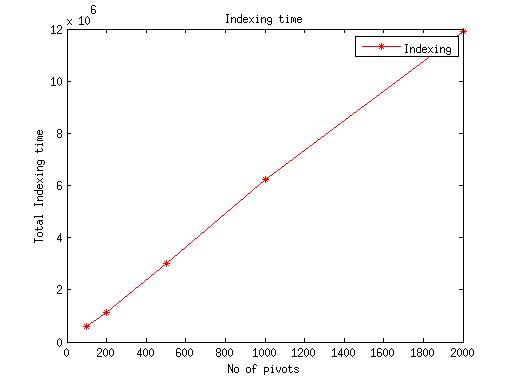
\includegraphics[width=0.35 \columnwidth]{img/indexing_time_n200k_d3_diffpivots.jpg}
\caption{Indexing time (in ms): As seen in the figure indexing time is increasing almost linearly with increase in the number of pivots chosen at each step of the M-tree algorithm. Even though indexing is an offline process we do not want the indexing time to run into days. If indexing time is very high, updates to the chemical compound database would be very expensive since we need a red-indexing into the chemical database. Hence we need to have a threshold for indexing time. The threshold distance used for this experiment was 0.3}
\end{figure}
%\pagebreak

\begin{figure}[ht]	
\centering
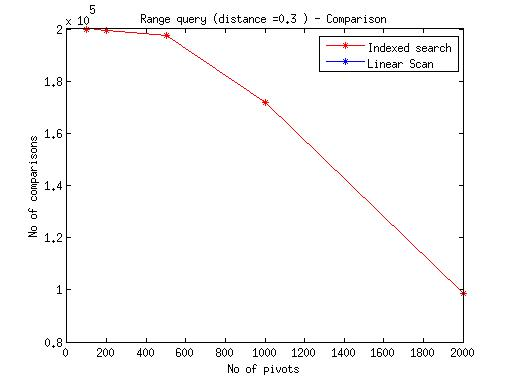
\includegraphics[width=0.35 \columnwidth]{img/comparisons_n200k_d3_diffpivots.jpg}
\caption{Comparisons: As seen in the figure, the number of comparisons i.e. the number of leaves containing chemical compounds which are visited in the M-tree index can be seen to decrease with increase in the number of pivots. We can notice that for number of pivots chosen as 2000, we are able to prune away more than half the nodes in the M-tree . The threshold distance used for this experiment was 0.3}
\end{figure}

\begin{figure}[ht!]	
\centering
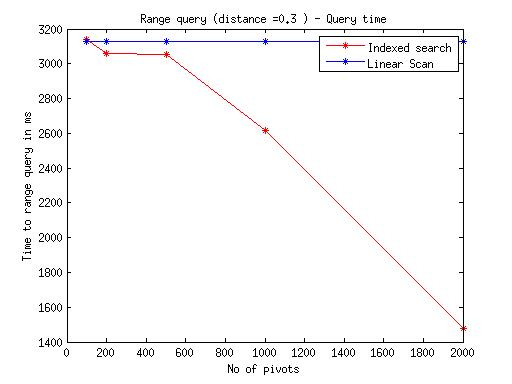
\includegraphics[width=0.35 \columnwidth]{img/query_time_n200k_d3_diffpivots.jpg}
\caption{Query time (in ms): As seen in the figure, the query time can be seen to decrease with increase in the number of pivots. For pivot set size of 2000 we are able to achieve more than 2-times speedup. The linear scan be seen to take about 3100 ms per compound our technique can be seen to take around 1500ms per second for the specific size of 2000 pivots.The threshold distance used for this experiment was 0.3}
\end{figure}


\subsection{Different outlier base size}

We observed that the outlier base size did not have a significant effect on the query time for range search or on number of comparisons. The indexing time increases with a lesser outlier base size because the depth of the M-tree increases . The algorithm is applied recursively on the outlier sets, hence when we have a lower base size limit for the outlier sets the number of times the recursion is applied is greater. Since we did not see a great change in query time or number of comparisons we have fixed the size the outlier size limit to 100 i.e the algorithm terminates when the outlier size becomes lesser than 100.

\subsection{Different distance range queries}

With increasing range distance query , we can see that  both the no of comparisons and query time increases with the distance. This is for a 100,000 data point set. The widely accepted similarity threshold cutoff using the Tanimoto distance is 0.3 which was used in the previous experiments. For lesser distance range queries we get a speed-up of more than 10 times. We have varied the threshold from 0.05 to 0.5 in steps of 0.05. It doesn't make sense to go beyond 0.5 since queries generally want to find similar compounds and 0.5 seems like the maximum threshold. We should expect the curve to fall beyond 0.5. This is because using the triangle inequality bounds, for higher values of threshold distacne we should be able include many subtrees in our answer without having to compare distance of query to all these points. 

\begin{figure}[ht!]	
\centering
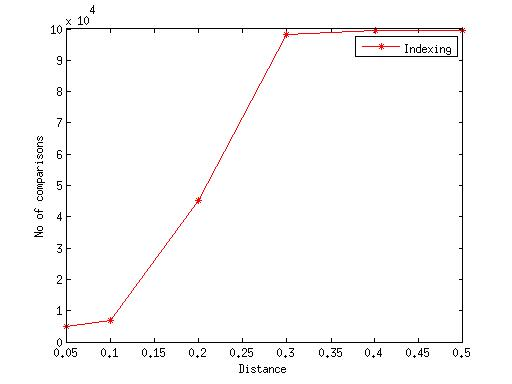
\includegraphics[width=0.35 \columnwidth]{img/comparisons_100k_500p_100o_differentdist.jpg}
\caption{Comparisons: The figure shows the number of comparisons made when different threshold values are used as similarity cutoff. As noticed in the figure, for lower values of threshold , pruning can be applied to more than 90 percent of the nodes . As the threshold reaches 0.5 very little pruning occurs.}
\end{figure}

\begin{figure}[ht!]	
\centering
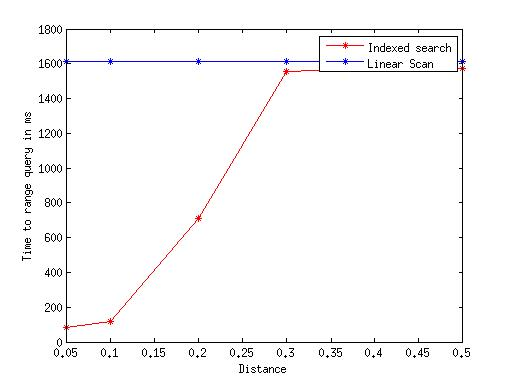
\includegraphics[width=0.35 \columnwidth]{img/query_time_100k_500p_100o_differentdist.jpg}
\caption{Query time (in ms): The figure shows the query time when different threshold values are used as similarity cutoff. As can be seen in the figure, for lower values of threshold almost 15 times speedup can be achieved though for threshold values close to 0.5 the query time increases and becomes comparable to the linear scan query time.}
\end{figure}
